\subsection{IFIT2-FLAG}
\subsubsection{Inpact of IFIT2-FLAG Expression in Mock Cells} \label{Inpact of IFIT2-FLAG Expression in Mock Cells}
\myparagraph{hi2f}
Cell Line: VERO \newline
Treatment: hIFIT2-FLAG \newline
Detecting magenta: exogenous human IFIT2 \newline
Detecting cyan: background \newline

This data is for comparison with bIFIT2-RNA-bingind mutant staining only. Some aggregations but the cells look reasonably healthy.

\begin{figure}
    \centering
    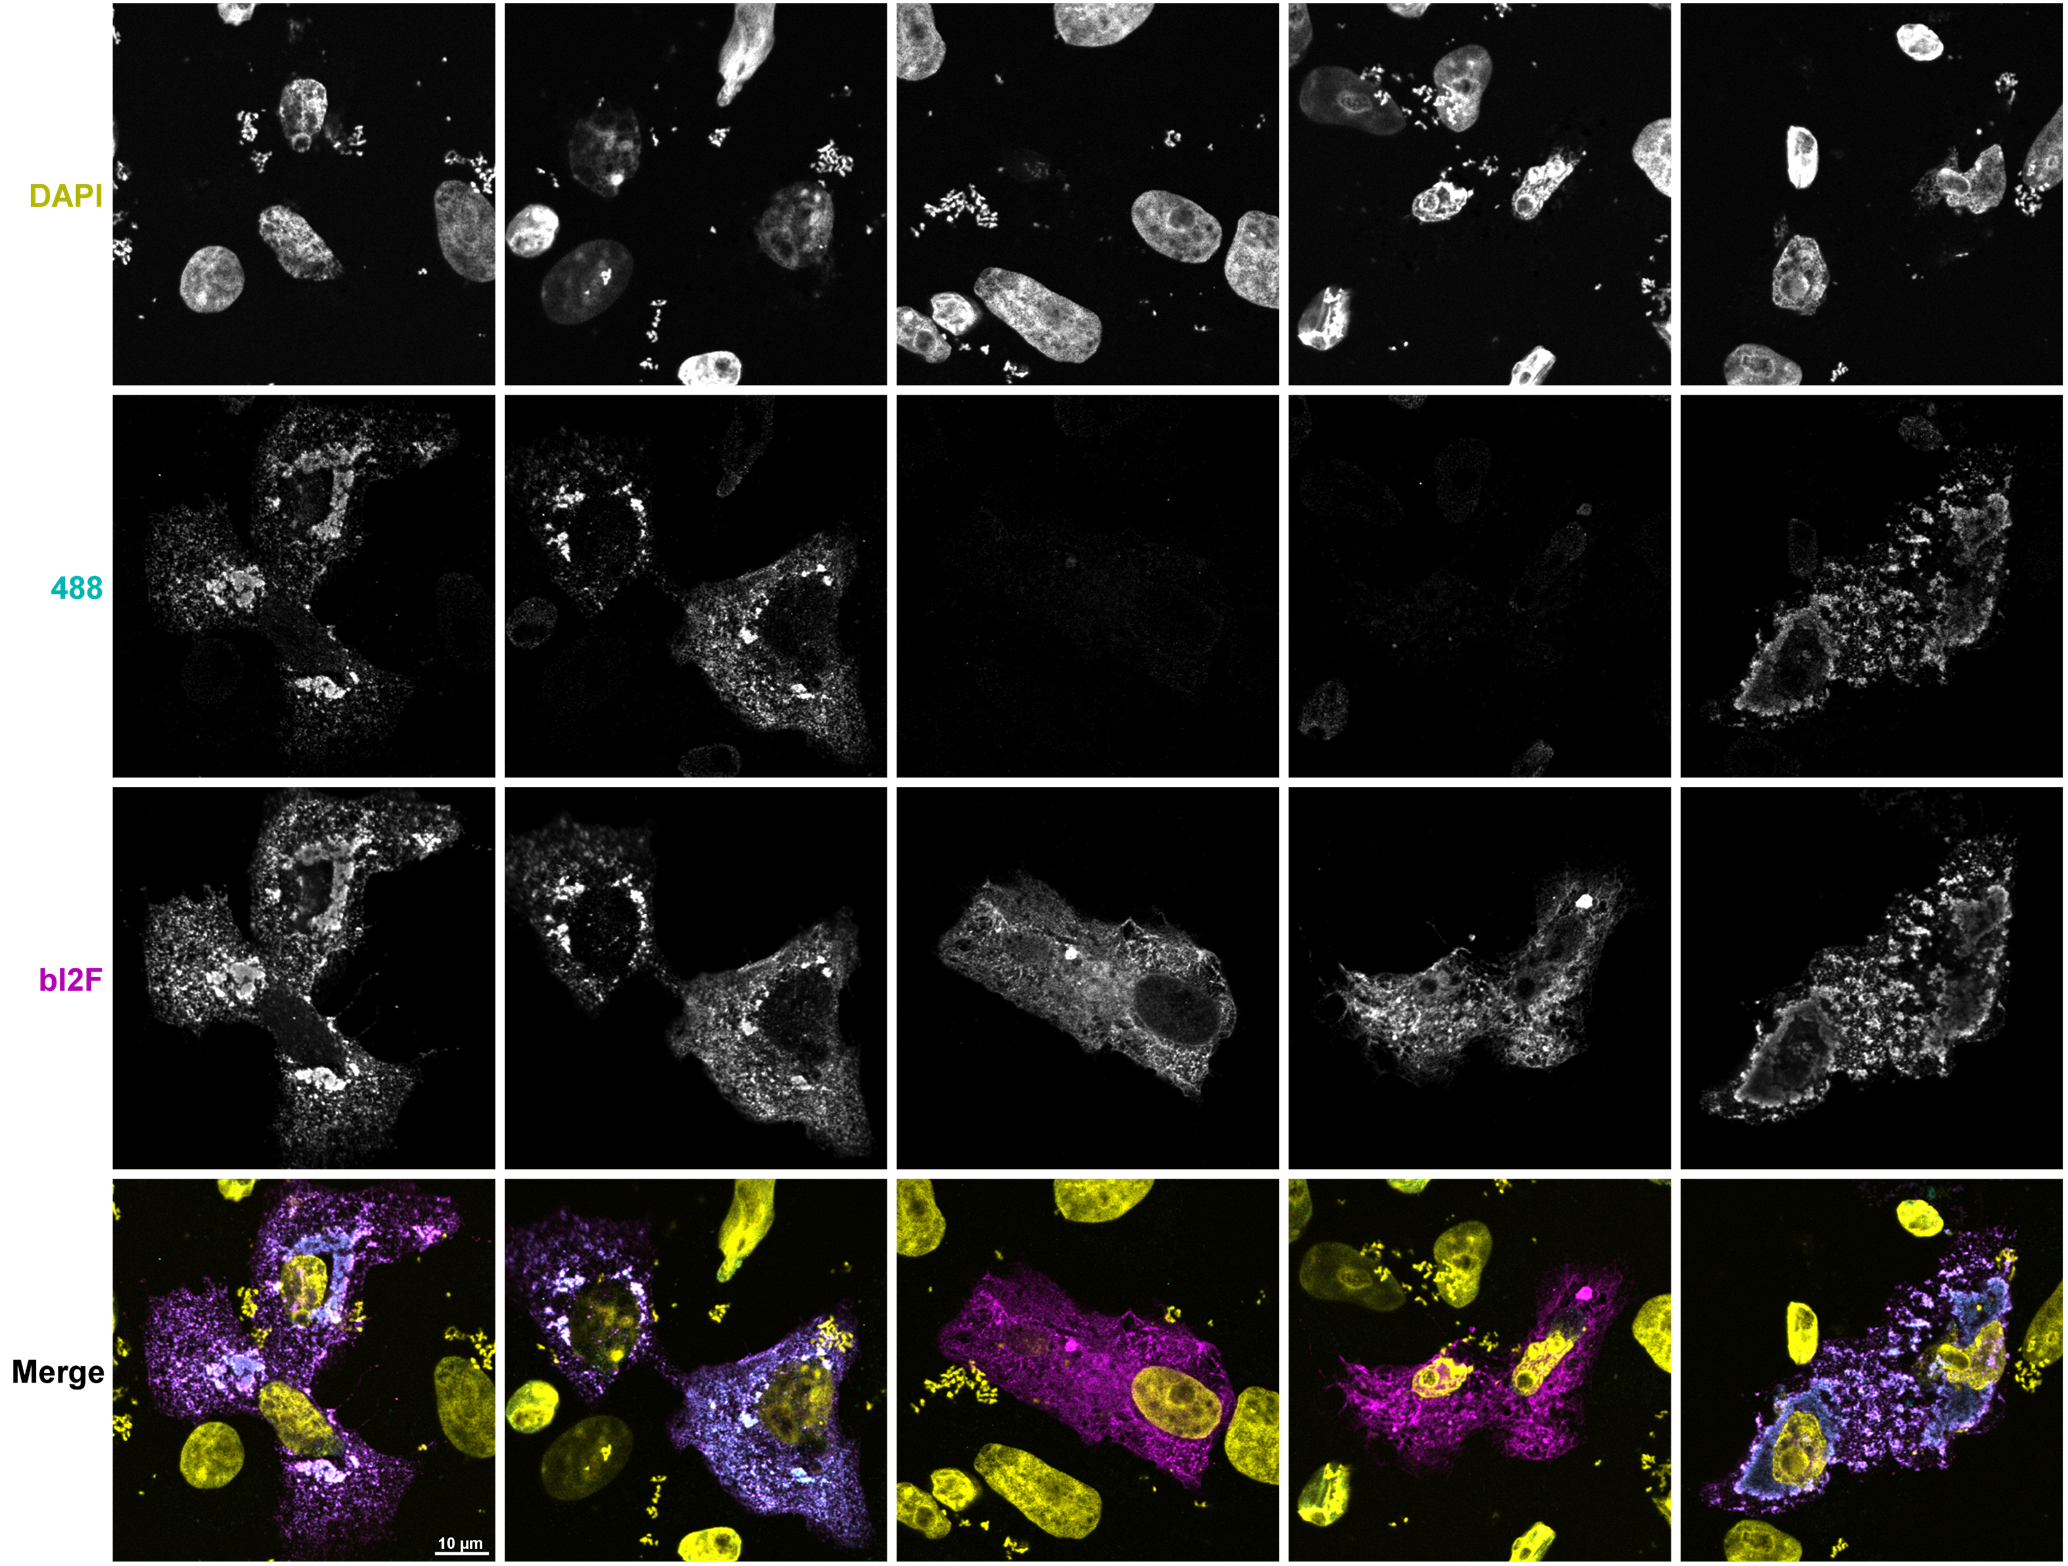
\includegraphics[width=1\linewidth]{10. Chapter 5//Figs//03. IFIT2-FLAG/01. hi2f mock.png}
    \caption[hi2f]{hi2f}
    \label{hi2f}
\end{figure}


\subsubsection{Exogenously Expressed IFIIT2-FLAG in a Simplified System of pseudo-IBs} \label{Exogenously Expressed IFIIT2-FLAG in a Simplified System of pseudo-IBs}
\myparagraph{hi2f hnhp}
Cell Line: VERO \newline
Treatment: hNhP + hIFIT2-FLAG \newline
Detecting magenta: exogenous human IFIT2 \newline
Detecting cyan: human pIB \newline

Exogenously expressed human IFIT2 colocalises with the pIB associated filamentous net (top panel). It also forms inclusion inside the human pIB structures. This data is consistent with what we observed with IFIT2A antibody. IFIT2 also seems to occasionally form aggregates/spots (highlighted by arrows). These could be functional or just aggregates caused by overexpression, we do not know.

\begin{figure}
    \centering
    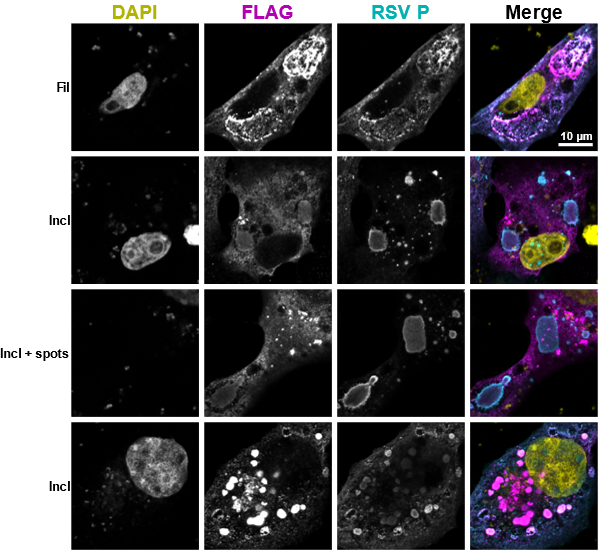
\includegraphics[width=1\linewidth]{10. Chapter 5//Figs//03. IFIT2-FLAG/02. hi2f hnhp.png}
    \caption[hi2f hnhp]{hi2f hnhp}
    \label{hi2f hnhp}
\end{figure}

\myparagraph{bi2f hnhp}
Cell Line: VERO hSLAM \newline
Treatment: hNhP + bIFIT2-FLAG \newline
Detecting magenta: exogenous bovine IFIT2 \newline
Detecting cyan: human pIB \newline

Exogenous bovine IFIT2 colocalises with the edge of human pIB structures. This is unusual as human IFIT2 data suggest inclusions with regards to pIBs.

\begin{figure}
    \centering
    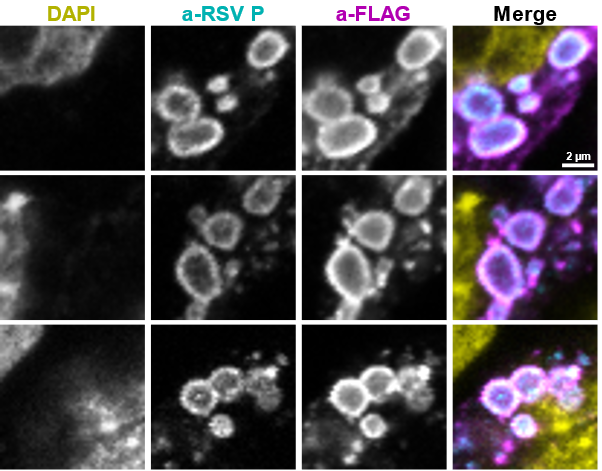
\includegraphics[width=1\linewidth]{10. Chapter 5//Figs//03. IFIT2-FLAG/03. bi2f bnbp.png}
    \caption[bi2f hnhp]{bi2f hnhp}
    \label{bi2f hnhp}
\end{figure}

\subsubsection{Exogenously Expressed IFIT2-FLAG During RSV Infection} \label{Exogenously Expressed IFIT2-FLAG During RSV Infection}
\myparagraph{hi2f hrsv}
Cell Line: VERO hSLAM \newline
Treatment: hRSV + hIFIT2-FLAG \newline
Detecting magenta: exogenous human IFIT2 \newline
Detecting cyan: human IB \newline

Overexpressed human IFIT2 during hRSV infection shows several phenotypes (in this experiment). We see IFIT2 being excluded from the IB interior while being concentrated to the IB ring (top panel); IFIT2 forming concentrated inclusion inside the IB structure (2nd panel); IFIT2 being excluded from the IB interior but colocalising to the IB ring and forming spots inside of the IB (3rd panel); and IFIT2 being diffused evenly through the cytoplasm and the IB structure (last panel). The different phenotypes suggest that IBs are dynamic structures, and the localisation depends on factors we do not comprehend yet. 

\begin{figure}
    \centering
    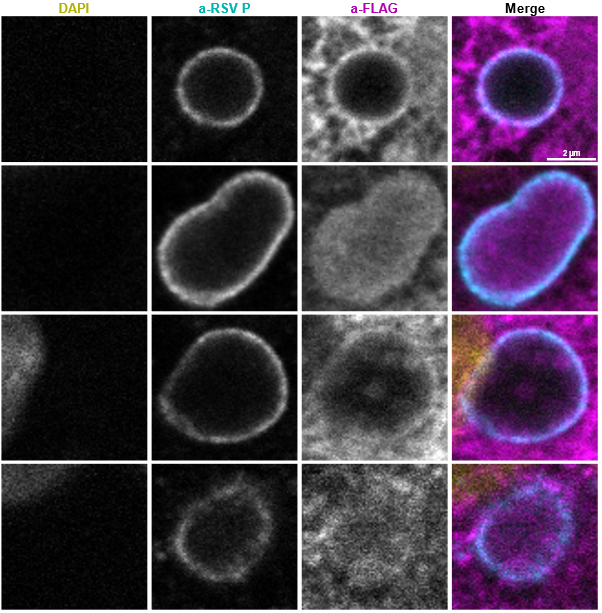
\includegraphics[width=1\linewidth]{10. Chapter 5//Figs//03. IFIT2-FLAG/04. hi2f hrsv.png}
    \caption[hi2f hrsv]{hi2f hrsv}
    \label{hi2f hrsv}
\end{figure}

\myparagraph{bi2f hrsv}
Cell Line: VERO \newline
Treatment: hRSV + bIFIT2-FLAG \newline
Detecting magenta: exogenous bovine IFIT2 \newline
Detecting cyan: human IB \newline

In the follow up experiment, exogenous bovine IFIT2 in the context of human RSV infection shows the same two phenotypes. It is either excluded from the IBs (middle panel) or colocalises with the ring structure of the IBs (top and bottom panel; highlighted with arrows).

\begin{figure}
    \centering
    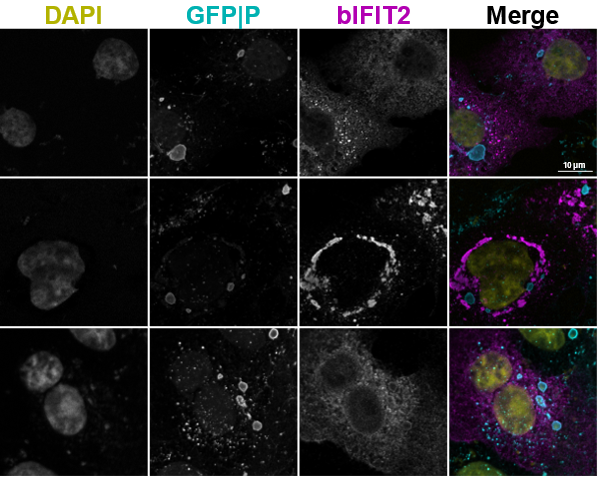
\includegraphics[width=1\linewidth]{10. Chapter 5//Figs//03. IFIT2-FLAG/05. bi2f hrsv.png}
    \caption[bi2f hrsv]{bi2f hrsv}
    \label{bi2f hrsv}
\end{figure}

\myparagraph{bi2f brsv}
Cell Line: VERO \newline
Treatment: bRSV + bIFIT2-FLAG \newline
Detecting magenta: exogenous bovine IFIT2 \newline
Detecting cyan: bovine IB \newline

Exogenous bovine IFIT2 during bovine RSV infection seems to be excluded from the inclusion bodies, although the data is not great and the IFIT2 is aggregated in both cells shown.

\begin{figure}
    \centering
    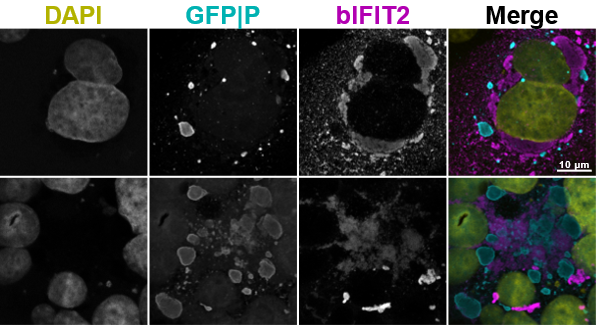
\includegraphics[width=1\linewidth]{10. Chapter 5//Figs//03. IFIT2-FLAG/06. bi2f brsv.png}
    \caption[bi2f brsv]{bi2f brsv}
    \label{bi2f brsv}
\end{figure}

\subsubsection{Summary} \label{Summary-i2-flag}
Overexpressing human IFIT2-FLAG does not seem to be detrimental to the cells. Exogenous human IFIT2 seems to form inclusions inside human pIB structures. It also colocalises with the pIB associated filamentous network. This data is consistent with IFIT2A antibody staining. IFIT2B staining showed inclusion inside pIB but failed to show the colocalization with the filamentous network. Exogenous bovine IFIT2 colocalises to the edge of human pIBs, which is in contrast to what we see with endogenous and exogenous human IFIT2 and its interaction with human pIBs. Exogenous human IFIT2 during human RSV infection showed different phenotypes in 2 different experiments. In the first experiment we observed it to: form inclusions inside the IB structure; be excluded from IB but colocalise to the IB ring; be excluded from the IB but colocalise to the ring and have spots inside the IB structure; or to be diffused through cytoplasm and IB equally. In the second experiment we observed it to be either completely excluded from the IBs or to colocalise with them. Exogenous bovine IFIT2 during human RSV infection was either completely excluded from the IB or was colocalised to the ring of the structure. This was consistently seen in both experiments conducted. Exogenous bovine IFIT2 during bovine RSV infection seems to be excluded from the IBs.